\begin{comment}
\end{comment}

\chapter{Circuits pour la tolérance aux fautes quantique}

Pour terminer le récit de ma thèse,
j'ajoute un niveau de réalisme au modèle de correction d'erreurs quantique
du chapitre précédent pour présenter la conception d'une mémoire quantique.
Une mémoire quantique est un système quantique permettant de stocker
de l'information pour une durée indéterminée.
Cependant,
tel que mentionné au chapitre précédent,
les systèmes quantiques sont sujets aux erreurs,
même lorsque aucune opération n'est effectuée.
Ainsi,
pour construire une mémoire quantique,
il est nécessaire, encore une fois,
d'utiliser un code correcteur pour corriger les erreurs au fur et à mesure
qu'elles affectent le système.
Du moins,
il faut s'assurer que les erreurs restent assez faibles afin de pouvoir utiliser
l'information stockée dans le système pour un calcul futur.

En principe,
il est possible d'utiliser n'importe quel code correcteur pour construire
une mémoire quantique,
mais certains ont des propriétées plus favorables.
D'abord,
il est difficile de mettre à l'échelle un code correcteur dont le graphe
de Tanner est local, soit un graphe où la distance entre chaque paire de sommets 
connectés par une arête est bornée indépendemment du nombre de sommets.
Plus précisément,
Bravyi, Poulin et Terhal~\cite{bravyi_tradeoffs_2010}
ont montré que pour un tel code $[n, k]$,
la distance minimale $d$ est limitée par
\begin{equation}
	d^2 \leq c \frac{n}{k},
\end{equation}
pour une constante $c$ indépendente de $n$, $k$ et $d$.
Ainsi,
si $k$ augmente proportionnellement avec $n$,
la distance minimale est bornée par une constante.
De plus,
pour avoir une distance minimale raisonnable,
il est nécessaire que le nombre de qubits encodés $k$ 
n'augmente pas ou très peu avec $n$.

Ce résultat implique que pour un grand $n$,
soit peu de qubits sont encodés,
soit ces derniers sont mal protégés des erreurs.
Il est donc difficile d'utiliser ces codes pour construire une mémoire 
quantique de grande taille.
Cependant,
lorsque la contrainte de localité du graphe de Tanner est abandonnée,
Gottesman~\cite{gottesman_fault-tolerant_2013} a montré qu'il est possible 
de construire une mémoire quantique protégeant efficacement les erreurs,
avec $\frac{k}{n}$ constant, en utilisant des codes LDPC.
Conséquemment,
il est possible d'utiliser des codes LDPC pour construire 
des mémoires quantiques de grandes échelles.

D'un point de vue expérimentale,
les codes LDPC ont l'avantages de pouvoir être implémentés de sorte que 
chaque qubit soit connecté à un nombre bornée d'autres qubits.
Comme je le présenterai plus tard lorsque j'introduirai les circuits
de mesures de syndromes,
cela permet d'implémenter efficacement les circuits nécessaires à la
construction d'une mémoire quantique,
à la condition de pouvoir coupler n'importe quelle paire de qubits 
indépendemment de la distance qui les sépare.

Comme les couplages à long portée sont difficiles pour plusieurs technologie de qubits,
il est tentant d'essayer d'implémenter des codes dont le graphe de Tanner est non local
à l'aide d'une architecture de qubits intéragissant localement,
quite à payer un léger surcout.
Cependant,
dans un article qui n'est pas présenté dans cette thèse~\cite{delfosse_bounds_2021},
Nicolas Delfosse, Michael Beverland et moi-même avons montré que le cout de cette approche
est en réalité beaucoup trop élevé.
Plus précisément,
nous avons montré que pour implémenter une mémoire à l'aide d'un bon code LDPC
avec un rendement $k/n$ constant,
le nombre total de qubits nécessaires $N$ et la profondeur du circuit $\tau$ sont 
bornée inférieurement par 
\begin{align}
	N^{1/2} \tau \geq c n,
\end{align}
où $c$ est une constante.
Ainsi,
soit un très grand nombre de qubits sont nécessaires,
soit le circuit doit être très long.
Dans les deux cas,
augmenter ces quantités offre plus d'occasions aux erreurs de ce manifester,
ce qui réduit significativement la qualité de la mémoire.

L'article présenté dans ce chapitre introduit une nouvelle architecture pour une mémoire quantique
qui permet d'implémenter des circuits pour de bons codes LDPC sans qu'il n'y ait de
croisement entre les couplages.
Bien que cela ne permet de régler le problème des couplages à long portée,
il s'agit d'un premier pas dans la bonne direction puisque les croisements
entre les couplages sont une limitation importante aux connections plus longues
pour plusieurs technologies de
qubits~\cite{sarovar_detecting_2020, debnath_demonstration_2016, neill_blueprint_2018, ash-saki_analysis_2020}.
De plus,
l'approche utilisée repose sur des algorithmes de tracé de graphes,
régulièrement utilisés pour l'intégration à très grande échelle de composante électronique
sur des puces classiques~\cite{leighton_complexity_1983},
mais jusqu'alors peu ou pas utilisés pour le design de systèmes quantiques.
Comme des expériences numériques démontrent le potentiel de cette approche pour la réduction
des erreurs dans une mémoire quantique,
les travaux de cet article ouvre la porte à utiliser d'avantage les méthodes 
de tracés de graphes pour la conception de systèmes quantiques.

Pour le reste de ce chapitre,
je présenterai d'abord les notions nécessaires de tolérance aux fautes et les modèles 
de bruits correspondant à une mémoire quantique.
Par la suite,
j'introduirai les codes de produits d'hypergraphes,
la famille de codes LDPC qui a été utilisée dans les expériences numériques,
avant de présenter l'article.

\section{Tolérance aux fautes quantique}

\section{Codes de produits d'hypergraphes et codes expanseurs}

\section{Article}

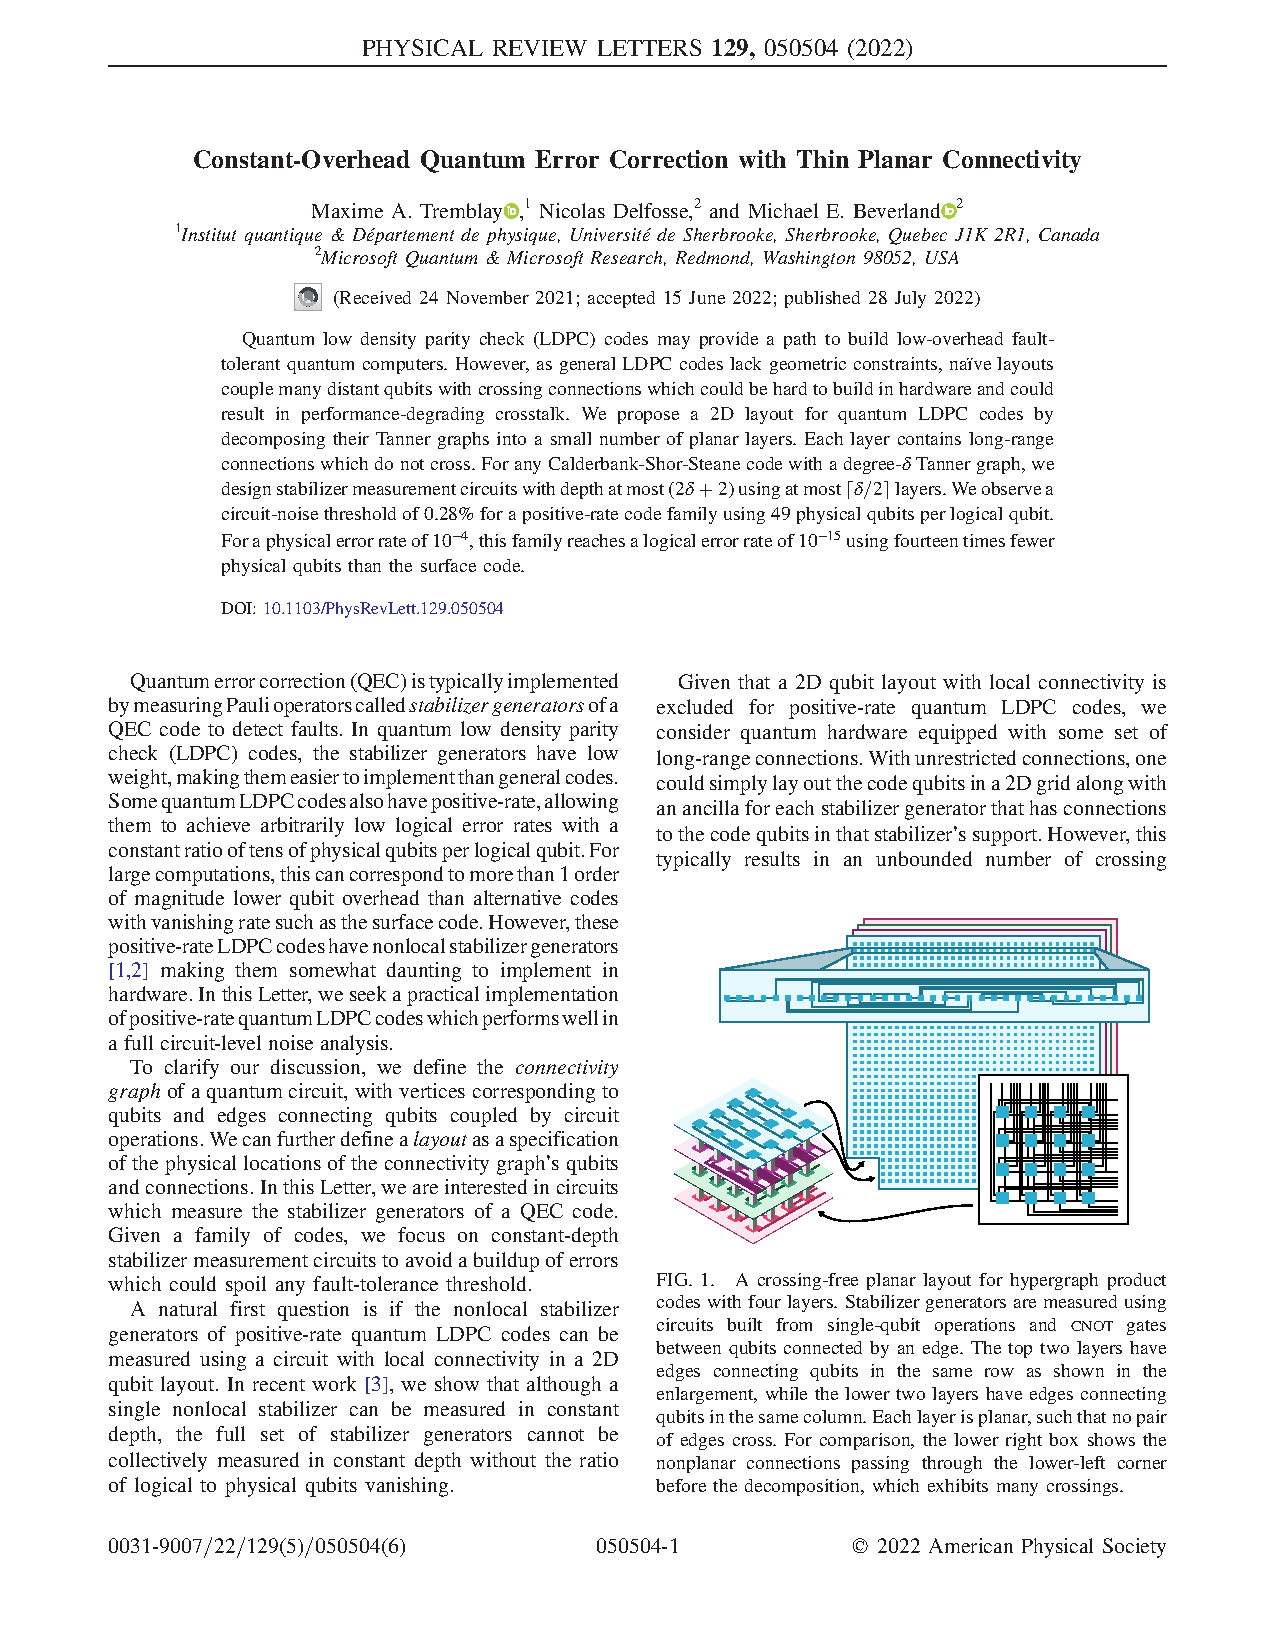
\includepdf[pages=-]{articles/planar_layout.pdf}

